\chapter{Methodology} \label{sec:matsmethods}
This chapter describes the data, methodology, and experimental setup used to develop and evaluate ATHENA. We first present the underwater image captioning dataset used for training and evaluation. We then describe the overall system architecture, including the image enhancement pipeline and VLM backbones. Finally, we detail the ablation study design, fine-tuning configurations, and evaluation metrics used to assess model performance.

\section{Data}

For our study, we use a publicly available underwater image captioning dataset collected by Huanyu et. al \cite{mainref}, which consists of 3,176 high-quality underwater images. We selected this dataset because it is the most comprehensive publicly available underwater dataset with multiple human-written captions per image. Other popular underwater datasets, such as UIEB \cite{uieb}, SQUID \cite{squid}, UID2021 \cite{uid}, URPC2021 \cite{urpc}, and DUO \cite{duo}, either lack captions, focus solely on object detection, or are much smaller in scale.

The images cover a wide range of resolutions and were resized to 224 × 224 pixels for consistency and ease of use. The dataset includes diverse underwater scenes, such as small distant targets, dense groups, visual blur, and low-light conditions, representing real-world underwater environments. The dataset also spans ten categories, predominantly fish (1861), coral reefs (1587), and divers (850).

Each image is annotated with five distinct captions provided by volunteers with domain expertise, resulting in a total of 15,880 captions. These captions, created as part of the original research, describe object morphology, color, quantity, motion, and additional scene context, ensuring rich vocabulary and syntactic diversity. Table~\ref{tab:examples}, adapted from Huanyu et al.~\cite{mainref}, presents some representative examples from the dataset.  The dataset provides a comprehensive benchmark for underwater scene understanding and forms the foundation for training and evaluating our vision-language model.

\begin{table}[htbp]
\centering
\caption{Sample images and captions from the dataset~\cite{mainref}}
\label{tab:examples} 
\begin{tabular}{>{\centering\arraybackslash}m{0.35\textwidth} m{0.55\textwidth}}
\toprule
\textbf{Image} & \textbf{Ground truth captions} \\
\midrule
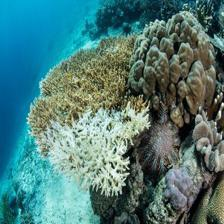
\includegraphics[width=0.33\textwidth]{figures/uic_img_5.jpg} & 
GT-1: Coral reefs in seawater come in a variety of colors, such as dark-brown, light-brown, and white. \newline
GT-2: An underwater coral reef full of life, with all kinds of corals growing freely. \newline
GT-3: Coral reefs in the water grow corals of various shapes and colors. \newline
GT-4: An undersea coral reef with corals of various colors and shapes. \newline
GT-5: There are many corals of various shapes and colors growing on the underwater reefs. \\
\midrule
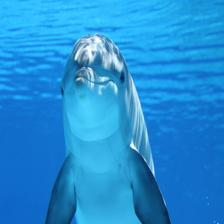
\includegraphics[width=0.33\textwidth]{figures/uic_img_6.jpg} & 
GT-1: A gray dolphin swims in the blue seawater. \newline
GT-2: There is a gray dolphin swimming at the bottom of sea. \newline
GT-3: A close-up of a dolphin swimming in the blue seawater. \newline
GT-4: There is a gray dolphin swimming in the seawater. \newline
GT-5: A gray dolphin swims at the bottom of sea. \\
\bottomrule
\end{tabular}
\end{table}

\section{Methodology}

\subsection*{System Architecture}
The ATHENA pipeline begins with image capture, sending the raw image and a system prompt as input. The image first passes through a multi-step enhancement pipeline, after which the enhanced image is fed into the VLM, which generates a structured textual description. Optional modules such as segmentation and retrieval-augmented grounding (RAG) can be integrated to mitigate hallucinations. The output text is then transmitted over a low-bandwidth acoustic channel to a remote operator. The overall architecture is illustrated in Figure~\ref{fig:athena_archi}.

\begin{figure}[h!]
    \centering
    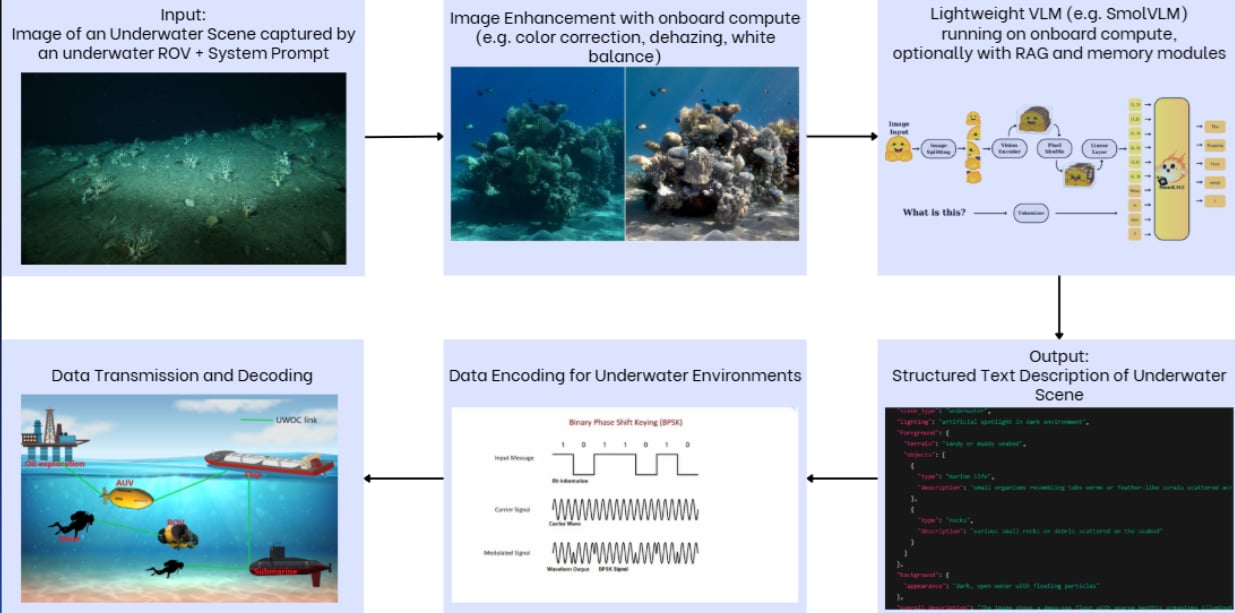
\includegraphics[width=\linewidth]{figures/athena_archi.jpeg}
    \caption{ATHENA system architecture}
    \label{fig:athena_archi}
\end{figure}

\subsection*{Image Enhancement Pipeline}
Raw underwater images are enhanced before VLM inference to improve feature extraction and caption accuracy. The pipeline is based on the seven-step protocol proposed by Wang et al.~\cite{7steppipeline}, with one modification: the original contrast stretching step is replaced with CLAHE for better local contrast enhancement~\cite{clahe}. The seven steps are: (1)~\textbf{Attenuated Channel Compensation (ACC)}, which restores absorbed reds and yellows; (2)~\textbf{White Balance} (YCbCr mean method), which corrects blue/green color casts; (3)~\textbf{Tone Mapping}, which enhances luminance across dark and bright regions; (4)~\textbf{HSL Saturation Adjustment}, which boosts color vividness; (5)~\textbf{CLAHE}, which improves local contrast without amplifying noise; (6)~\textbf{Gamma Correction}, which adjusts brightness for under- and overexposed regions; and (7)~\textbf{High-Pass Fusion}, which sharpens edges and fine details for better VLM feature recognition. These steps address three main visual issues: the first four correct color distortions, the next two enhance contrast, and the final step sharpens image details. The overall process is illustrated in Figure~\ref{fig:pipeline}.

\begin{figure}[ht]
    \centering
    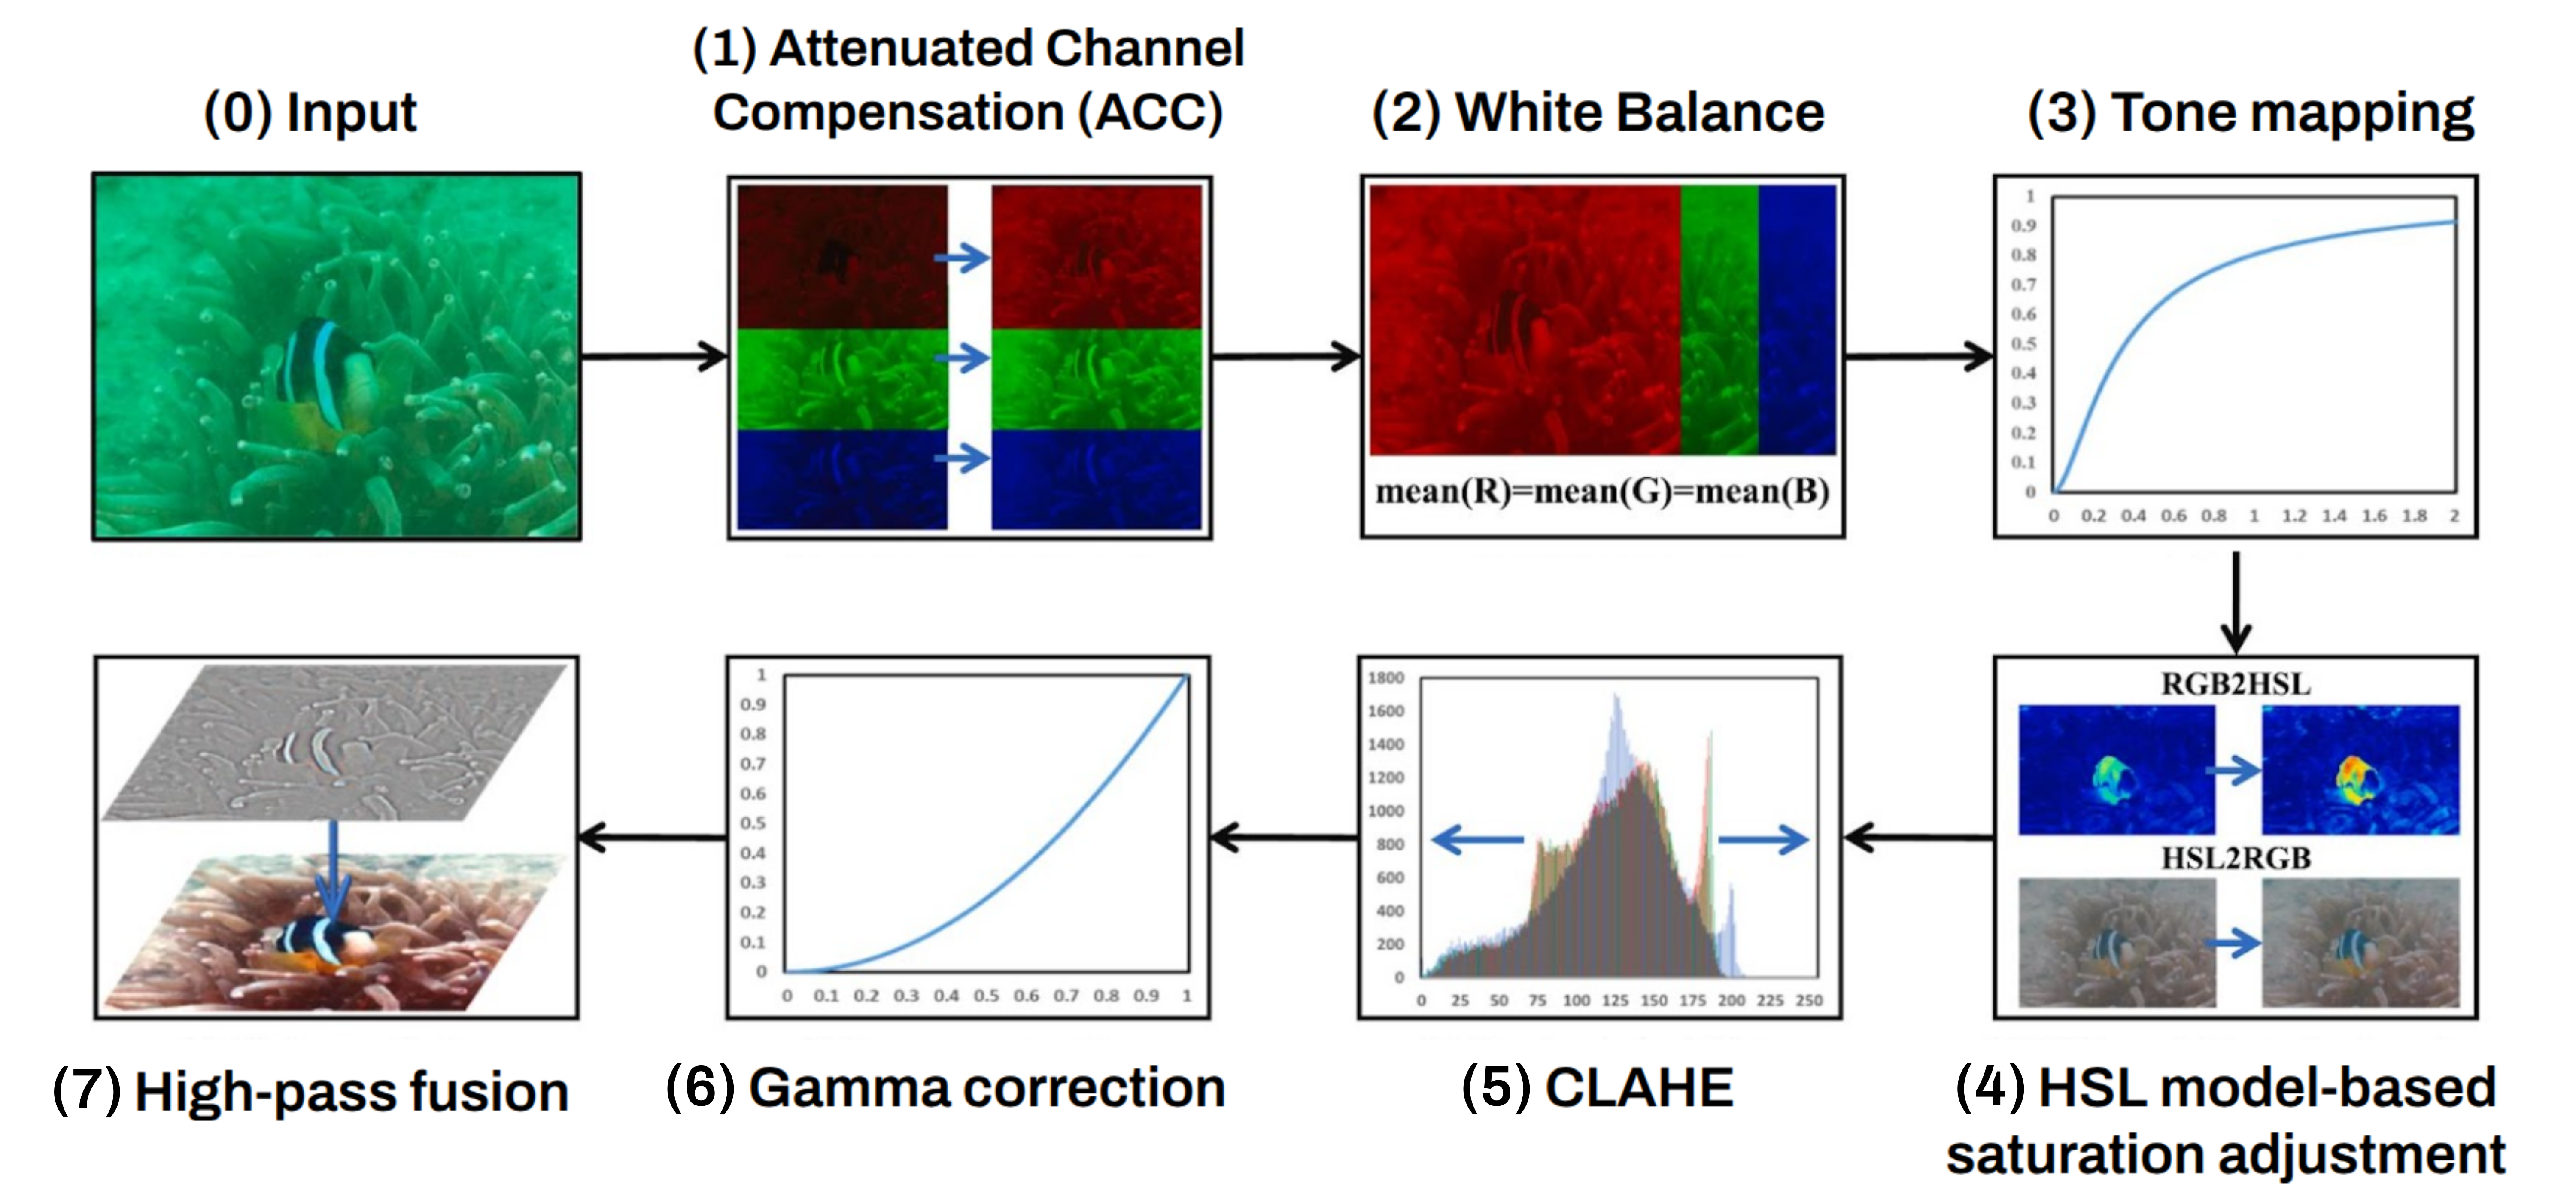
\includegraphics[width=\linewidth]{figures/revised-pipeline.png}
    \vspace{2mm}
    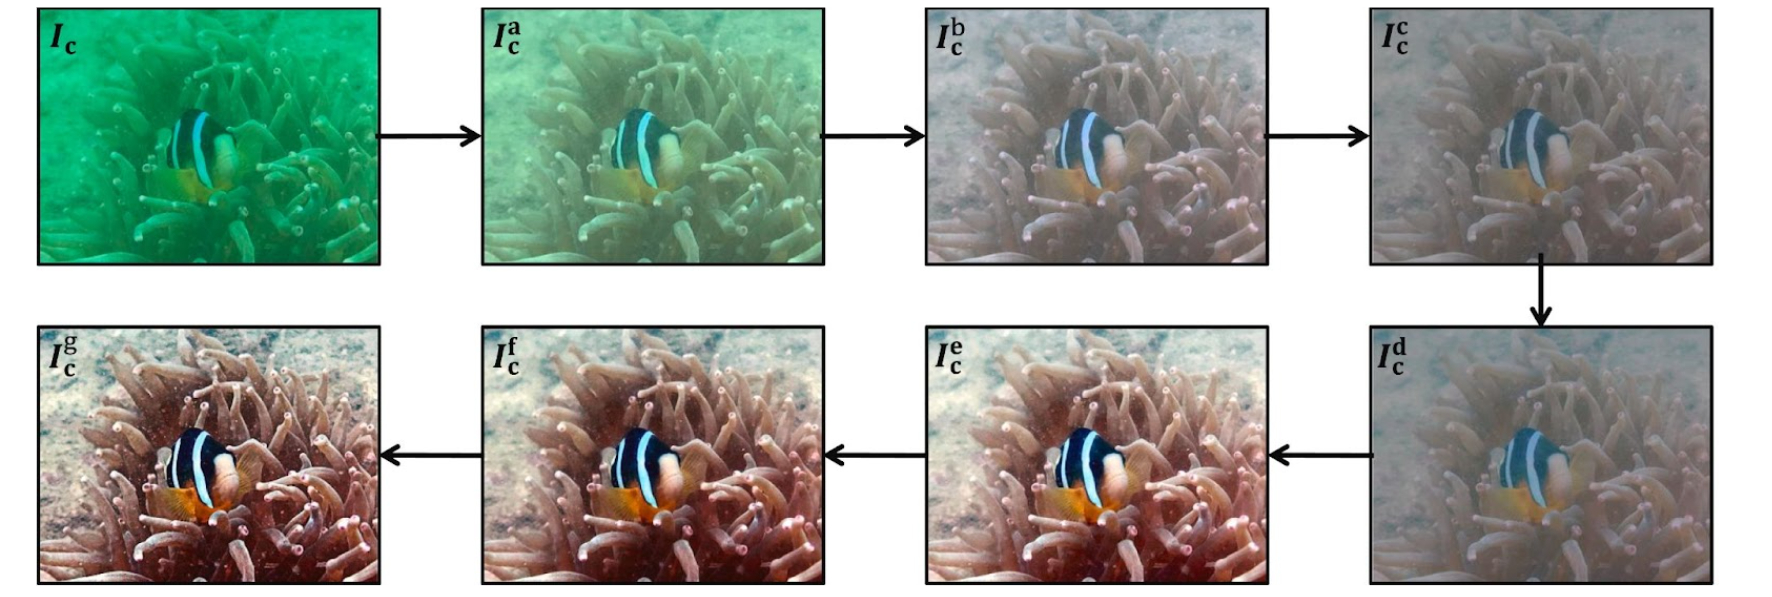
\includegraphics[width=\linewidth]{figures/pipeline-sample.png}
    \caption{Image enhancement pipeline (top) and sample output (bottom)}
    \label{fig:pipeline}
\end{figure}

\subsection*{VLM Backbone Selection}
\label{sec:backbone}
Three VLM backbones of varying architectural scales are evaluated to identify the most suitable model for underwater scene captioning under resource constraints. \textbf{SmolVLM-Instruct}~\cite{marafioti4} represents the lightweight end, offering a sub-1\,GB memory footprint suitable for real-time onboard inference. \textbf{BLIP-2 OPT 2.7B}~\cite{blip2} serves as an intermediate-scale reference with strong zero-shot captioning potential but known limitations in linguistic consistency~\cite{hani2026systematic}. \textbf{Qwen3.5}~\cite{tensorrt} represents the large-scale upper bound, with stronger scene understanding capabilities and support for embedded inference via NVIDIA TensorRT Edge-LLM. Parameter-efficient fine-tuning is applied to all three backbones using Low-Rank Adaptation (LoRA)~\cite{lora} and Weight-Decomposed Low-Rank Adaptation (DoRA)~\cite{dora}. DoRA extends LoRA by decomposing pretrained weights into magnitude and directional components, more closely resembling full fine-tuning behavior without additional inference overhead~\cite{dora}. Each backbone is evaluated across three LoRA ranks ($r = 8, 16, 32$) with DoRA enabled and disabled, yielding six configurations per backbone and 18 total, as summarized in Table~\ref{tab:ablation}.

\begin{table}[h]
\centering
\caption{Ablation study configurations}
\label{tab:ablation}
\begin{tabular}{lccc}
\hline
\textbf{VLM Backbone} & \textbf{LoRA Rank} & \textbf{DoRA} & \textbf{Configs} \\
\hline
SmolVLM-Instruct  & 8, 16, 32 & True / False & 6 \\
BLIP-2 OPT 2.7B   & 8, 16, 32 & True / False & 6 \\
Qwen3.5           & 8, 16, 32 & True / False & 6 \\
\hline
\textbf{Total}    &           &              & \textbf{18} \\
\hline
\end{tabular}
\end{table}

For all configurations, an alpha of 17 and a dropout rate of 0.05 were used, and the vision encoder was frozen during training.

\section{Experiments}

\subsection*{Evaluation Metrics}
Model performance is assessed using standard captioning metrics: BLEU-1 through BLEU-4~\cite{bleu}, which measure $n$-gram overlap (unigram to 4-gram) between predicted and reference captions; ROUGE-L~\cite{rouge}, which captures sentence-level structural similarity via longest common subsequence; and CIDEr~\cite{cider}, which rewards consensus with multiple human references. Scores range from 0 to 1 for BLEU and ROUGE-L, and 0 to 5 for CIDEr, with higher values indicating better agreement with human-annotated captions.

\subsection*{Implementation Details}
ATHENA is implemented using PyTorch and the HuggingFace Transformers library. All images are resized to $224 \times 224$ pixels and processed through the enhancement pipeline before training and inference. All three backbones are evaluated under the same dataset, enhancement pipeline, and training procedure to ensure fair comparison. All models are fine-tuned for 3 epochs using the 8-bit Paged AdamW optimizer with a learning rate of $2 \times 10^{-4}$ and a cosine learning rate scheduler with 100 warmup steps. A per-device batch size of 2 with 8 gradient accumulation steps yields an effective batch size of 16. Fine-tuning and experiments are conducted on an NVIDIA A100 40\,GB GPU using Flash Attention 2. The following custom system prompt is used during training for all configurations: \textit{``You are a VLM attached to an underwater robot. Describe the scene. Be concise but thorough.''} To assess deployment feasibility, all backbones are quantized to 4-bit NF4 format using the \textit{bitsandbytes} library and served via a \textit{FastAPI} server, and their VRAM footprints and inference latencies are recorded.
